\begin{figure}
    \centering
    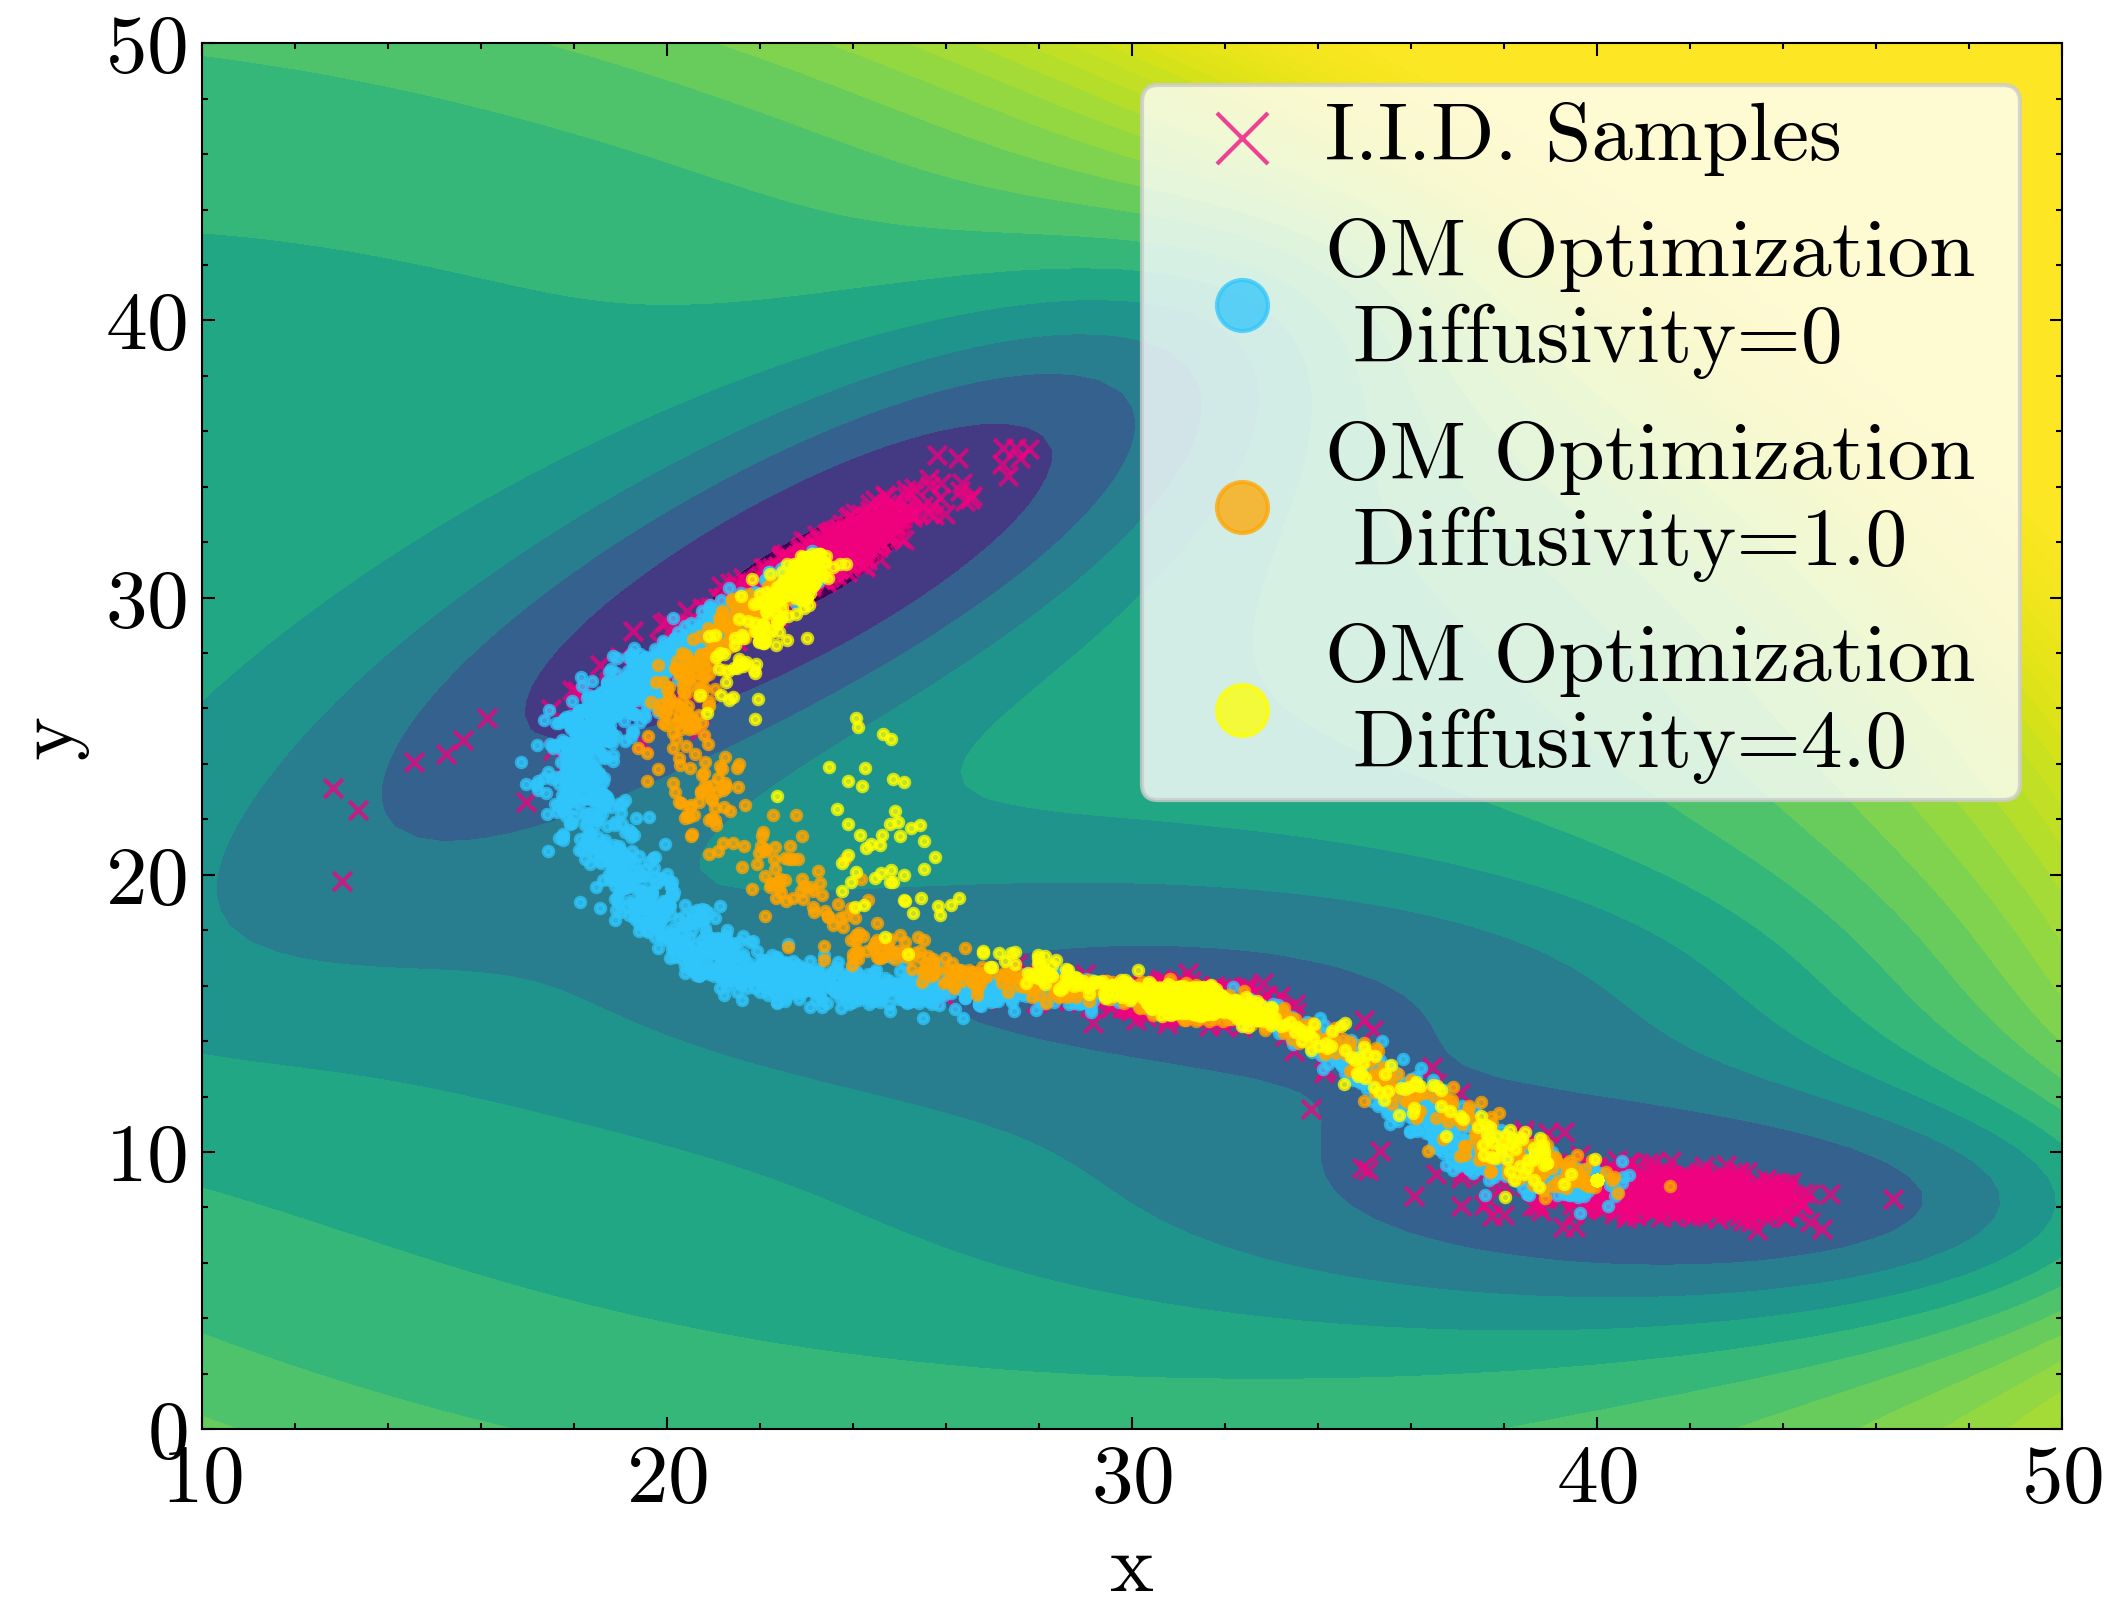
\includegraphics[width=\linewidth]{Figures/hessian_mb_contour_old_params.png}
    \caption{\textbf{OM optimization with a diffusion model on the 2D Müller-Brown potential.} Individual points along the OM-optimized paths are shown as dots. Increasing the diffusivity $D$ causes the path to cross at a higher barrier. An equivalent number of I.I.D samples (red) fails to sample the transition region. }
    \label{fig:mb_hessian_diff}
\end{figure}
\begin{figure}
    \centering
    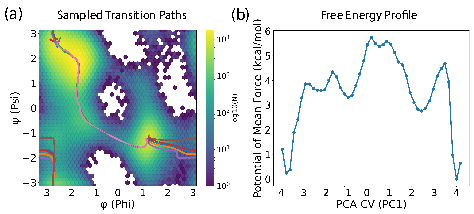
\includegraphics[width=1.0\linewidth]{Figures/ala_free_energy.pdf}
    \caption{\textbf{OM optimization and free energy barrier estimation on alanine dipeptide using a pre-trained diffusion model.} \textbf{(a)} Sampled alanine dipeptide transition paths from OM optimization with a pretrained diffusion model, overlaid on a Ramachandran plot of sample density at 600K. \textbf{(b)} Free energy barrier for a selected path, estimated via umbrella sampling, is approximately 6 kcal/mol, in line with our metadynamics calculations (\ref{sec:alanine_dipeptide_details}).}
    \label{fig:free_energy}
\end{figure}
\vspace{-5pt}
\begin{table}[t]
\caption{\textbf{Benchmarking the speed of OM optimization against traditional enhanced sampling baselines on alanine dipeptide.} We report the number of force field evaluations required per 1,000 step transition path (for OM optimization we instead report the number of score function evaluations). OM optimization requires significantly fewer evaluations and thus lower computational cost per path than the traditional approaches.}
\label{tab:ala_method_comparison}
\scriptsize
\centering
\resizebox{\columnwidth}{!}{%
\begin{tabular}{llll}
\toprule
\textbf{Method} & \textbf{CVs} & \textbf{\# FF Evals / Path ($\downarrow$)} & \textbf{Runtime / Path} ($\downarrow$)\\
\midrule
\textbf{MCMC (Two-Way Shooting)} & No & $\geq$ 1B & $\geq$ 100 hours\\
\textbf{Metadynamics} & Yes & 1M & 10 hours\\
\textbf{OM Opt. (Diffusion Model) (ours)} & No & \textbf{10K} & \textbf{50 min}\\
\bottomrule
\end{tabular}%
}
\end{table}
\vspace{-5pt}
\begin{figure*}[h]
    \centering
    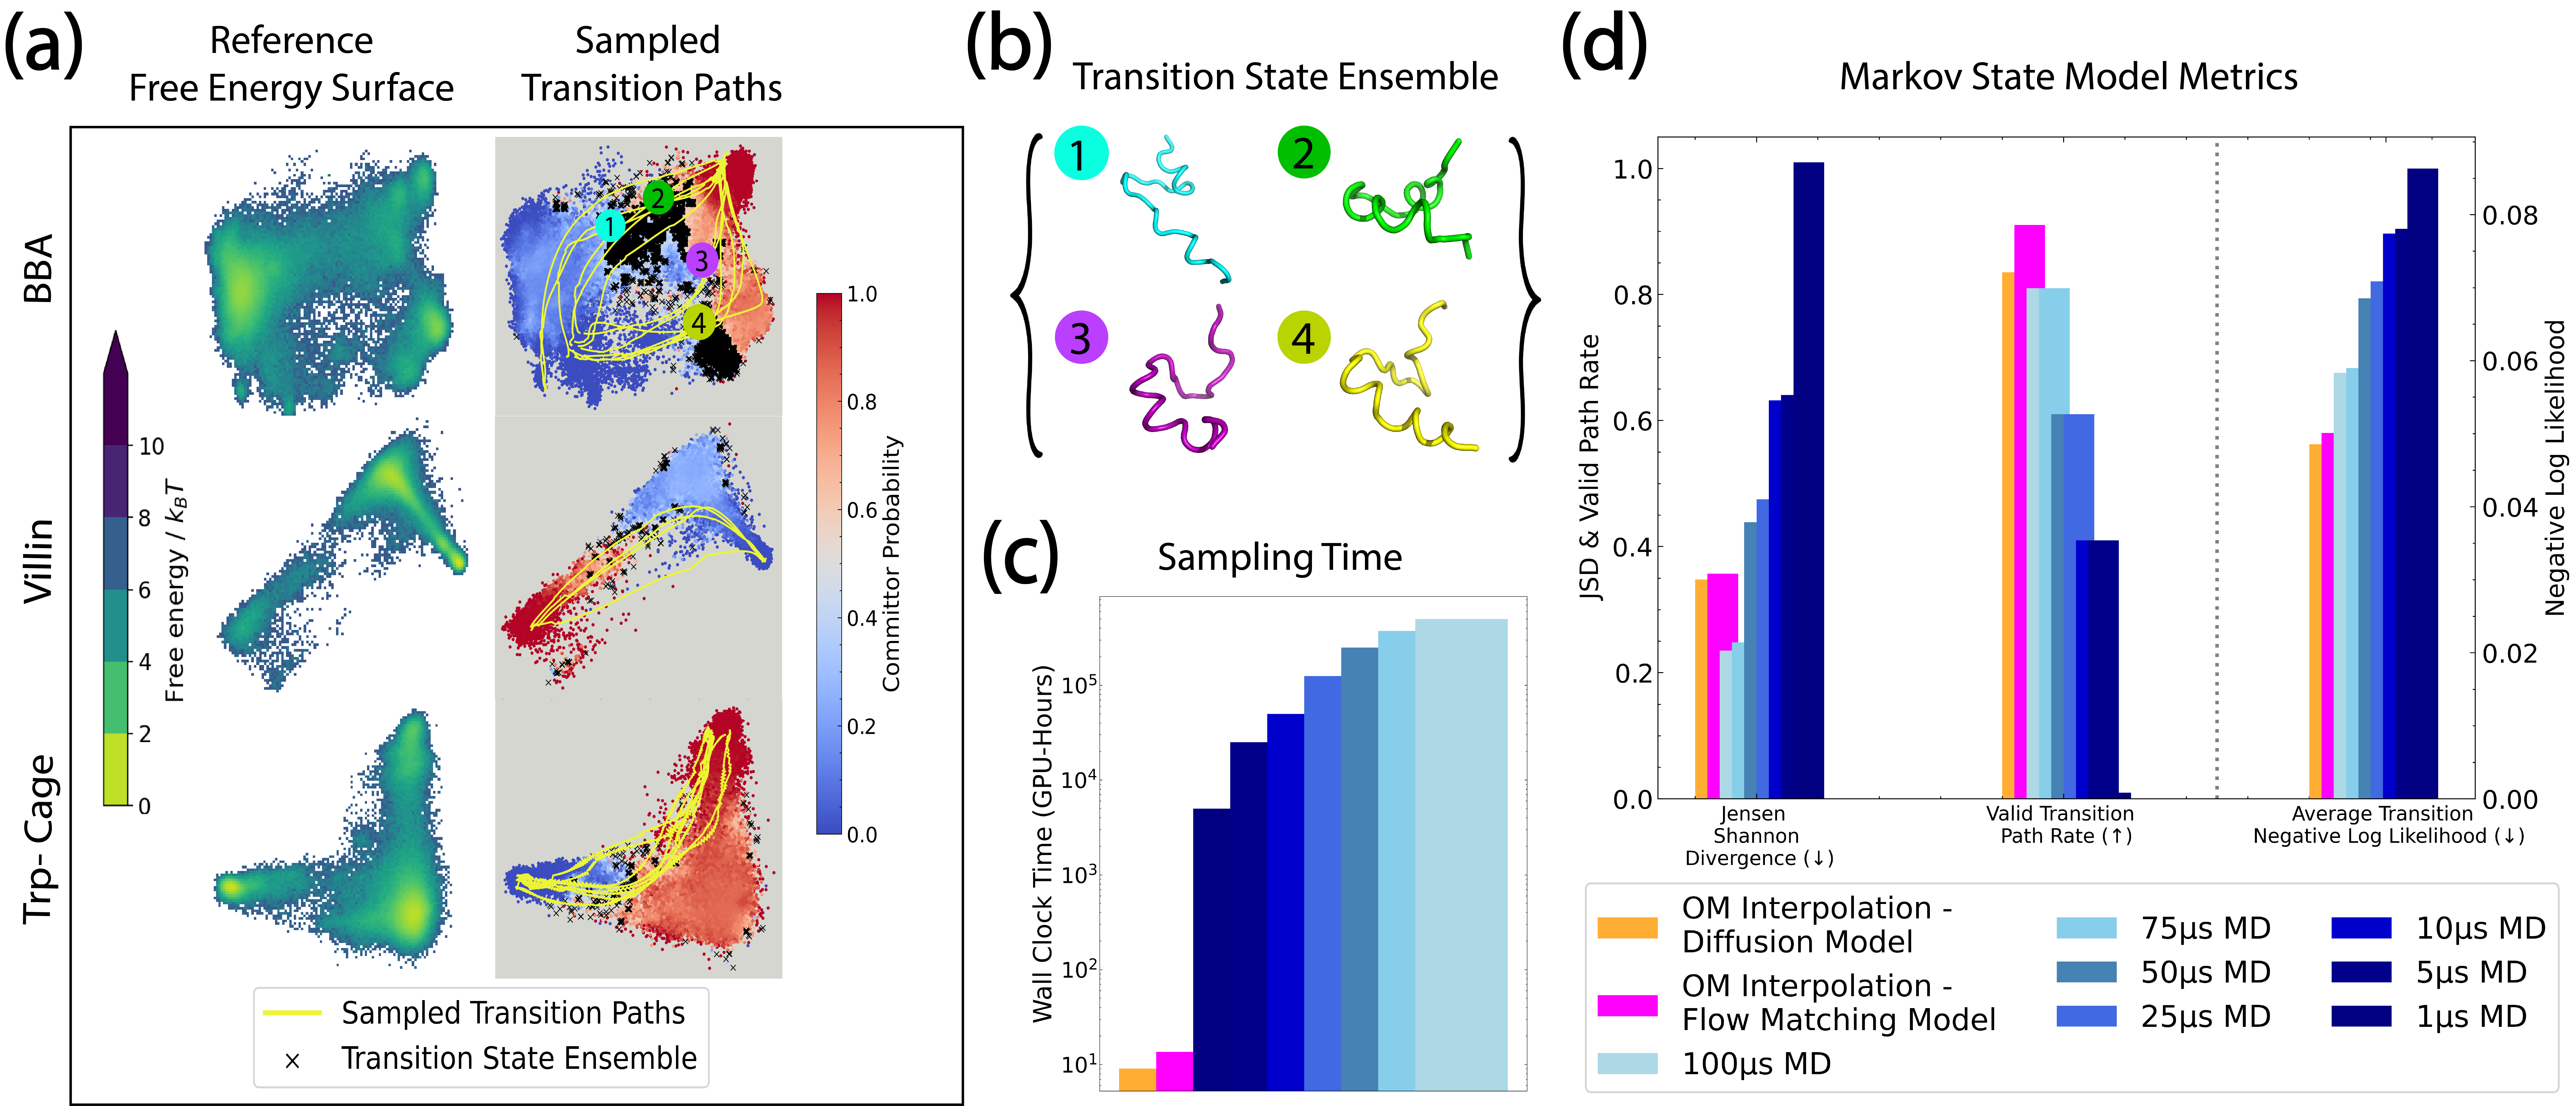
\includegraphics[width=1.0\linewidth]{Figures/fastfolders_figure.png}
    \caption{\textbf{OM optimization with diffusion and flow matching models trained on coarse-grained, fast-folding proteins.} \textbf{(a)} Reference free energy surfaces of fast-folding proteins, alongside transition paths produced by OM optimization (yellow) overlaid against the landscape of the empirically computed committor function $q(\xx)$. The transition state ensemble (black) is the set $\left \{ \xx : 0.45 \leq q(\xx) \leq 0.55 \right \}$. \textbf{(b)} Samples from the predicted transition state ensemble of BBA. \textbf{(c)} Runtime of OM optimization and varying lengths of unbiased MD simulation of BBA. MD simulation is performed with the diffusion model score as an approximate force field, as in \citet{arts2023two}. \textbf{(d)} MSM results averaged across 5 fast-folding proteins. Comparisons are with respect to reference, unbiased MD simulation of varying lengths. Plotted are the Jensen-Shannon Divergence (a measure of distributional dissimilarity) between the sampled and reference path MSM state distributions, fraction of sampled paths which are valid (i.e., have non-zero probability under the reference MSM), and average transition negative log likelihood under the reference MSM (indicating the realism of the paths).}
    \label{fig:fastfolders}
\end{figure*}
\section{Results}
We now present the results of our OM optimization approach for TPS with pre-trained generative models. In all cases other than the Müller-Brown potential (\sref{sec:mb_results}), we perform OM optimization in configuration space, so we skip the final decoding step and use physical parameter values. In Appendix \ref{sec:classical_ff}, we demonstrate a use case beyond generative modeling, namely using a classical force field to generate all-atom transition paths for Chignolin and Trp-Cage. 
\vspace{-5pt}
\subsection{2D Müller-Brown potential}
\label{sec:mb_results} 
% \begin{table*}
% \caption{Comparison of transition path sampling methods on the 2D Müller-Brown potential. NFE is the number of potential evaluations required to sample 1,000 paths \sr{How do we know how much MD to perform after OM optimization?} \sr{Also, can we diversify the MB paths by picking random points in the two wells instead of a single endpoint?}}
% \label{tab:mb_results}
% \scriptsize
%     \begin{tabular}{lccccc}
%         \toprule
%         Method & RMSD (Å) ↓ & THP (\%) ↑ & ETS (kJ/mol) ↓ & NFE ↓ \\
%         \midrule
%         Unbiased MD (300K) & & & & & \\
%         Unbiased MD (700K) & & & & & \\
%         DiffSim \cite{sipka2023differentiable} & & & & & \\
%         Doob's Lagrangian \cite{du2024doob} & & & & & \\
%         OM (Data Free) (ours) & & & & & \\
%         OM (diffusion Model) (ours) & & & & & \\
%         OM (Flow Model) (ours) & & & & & \\
%         \bottomrule
%     \end{tabular}
% \end{table*}
\vspace{-5pt}
We first demonstrate our method on the 2D Müller-Brown (MB) potential \cite{muller1979location}, a canonical test system for TPS with a global minimum and two local minima, separated by saddle points.
\vspace{-10pt}
\paragraph{Problem setup.} Using a denoising diffusion model pretrained on samples from the underlying potential energy surface, we generate transitions between the two deepest energy minima using OM optimization. We generate the initial guess path via linear interpolation at $\tau_\text{initial} = 8$ (the maximum diffusion model time is $T_d = 1,000$). We perform 200 steps of OM optimization directly at $\tau_\text{initial} = 8$ using $\tau_\text{opt} = 8$, and finally decode the path back to the data distribution via the denoising process. 
\vspace{-5pt}
\paragraph{Results.} As shown in \fref{fig:mb_hessian_diff}, OM optimization with the truncated action yields a transition path (shown in blue) between the energy minima which passes through the lowest energy barrier. Due to the stochastic decoding process, the samples around the transition path exhibit natural diversity. Increasing the diffusion coefficient $D = \frac{k_BT}{\gamma M}$ results in qualitatively different transition paths (shown in orange and yellow). Samples are more concentrated in the three energy minima, and the path crosses a higher energy barrier, consistent with the larger scale of thermal fluctuations at increased temperatures. Meanwhile, 2500 i.i.d. samples (shown in red) from the diffusion model sample only the three energy minima, and fail to sample the transition region. This provides a proof-of-concept that our OM optimization procedure can be used to repurpose generative models to sample transition paths without specialized training. See Appendix \ref{sec:mb_details} for additional results and analysis on the MB potential, including with a flow matching model.
\vspace{-5pt}
\paragraph{Committor and Transition Rate Estimation.} Committor functions and rates are fundamental quantities in the study of transition events \cite{vanden2006towards}. The committor function $q(\xx)$ is defined as the probability that a trajectory initiated at $\mathbf{x}^{(0)} = \mathbf{x}$ reaches the target state $\mathcal{B}$ before the starting state $\mathcal{A}$. Transition paths obtained via OM optimization can be used as an enhanced sampling method to accurately compute the committor function, and subsequently the transition rates, on the Müller-Brown potential (see Appendix \ref{sec:mb_details} for complete details). Specifically, we initiate MD simulations from points along the OM-optimized paths shown in \fref{fig:mb_hessian_diff} to collect a dataset of samples $\mathcal{D}_\text{train}$. We then train a committor function $q_\theta(\xx)$ by solving a functional optimization problem given by the Backward Kolmogorov Equation (BKE) over the sampled points, and finally compute an estimate of the reaction rate using the trained model via the relation \cite{vanden2006towards}:
\begin{equation}
\label{eq:final_rate}
    k_\theta = \frac{k_BT}{\gamma}\langle |\nabla_\xx q_\theta(\xx)|^2 \rangle_\Omega \approx \hat{\mathbb{E}}_{\xx \sim \mathcal{D}_\text{train}} |\nabla_\xx q_\theta(\xx)|^2,
\end{equation}
where $\langle \cdot \rangle_\Omega$ denotes an ensemble average over the configurational space $\Omega$ and $\hat{\mathbb{E}}$ denotes an empirical mean . Using this procedure, we obtain a transition rate estimate of $1.3 \times 10^{-5}$, compared with the true rate of $5.4 \times 10^{-5}$. It is often challenging to compute the reaction rate even within the correct order of magnitude \cite{rotskoff2022active, hasyim2022supervised}, suggesting the promise of our OM optimization method to enable accurate rate estimation on more challenging systems.
\vspace{-5pt}
\subsection{Alanine dipeptide}
\label{sec:alanine_dipeptide_results}
Alanine dipeptide is a classic benchmark system for TPS, with 22 atoms and CVs described by the dihedral angles $\phi, \psi$. 
\vspace{-5pt}
\paragraph{Problem setup.} We start with a denoising diffusion model pre-trained on samples from the alanine dipeptide potential energy surface. Using this model, we perform OM optimization to find transition paths between the two standard minima defined in the CV space. 
\vspace{-10pt}
\paragraph{Results.} We successfully sample two likely transition paths between the metastable basins (\fref{fig:free_energy}a). In Table \ref{tab:ala_method_comparison}, we benchmark the computational efficiency of OM optimization against traditional enhanced sampling techniques, namely metadynamics \cite{laio2008metadynamics} and MCMC-based two-way shooting \cite{bolhuis2021transition}, and find that OM optimization is considerably more efficient. As shown in \fref{fig:free_energy}b, we can also use the transition paths resulting from OM optimization as a natural CV for umbrella sampling \cite{torrie1977nonphysical}, from which we can accurately and efficiently estimate free energy profiles along the transition path. See Appendix \ref{sec:alanine_dipeptide_details} for complete details on model training, OM optimization, and free energy calculations. 
\begin{figure}[t]
    \centering
    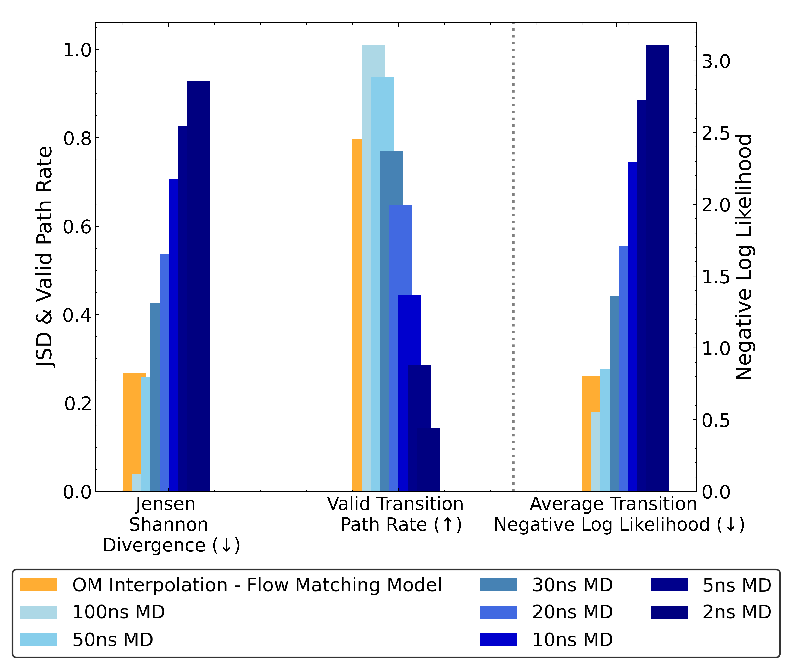
\includegraphics[width=1.0\linewidth]{Figures/tetra_figure_all_atom.pdf}
    \caption{\textbf{OM optimization on unseen tetrapeptide sequences.} OM optimization with a flow matching model yields transition paths which compare strongly with variable-length MD simulations, indicating the generalization potential of our approach. Plotted are the Jensen Shannon Divergence (a measure of distributional dissimilarity) between state distributions visited by the reference and generated paths, the fraction of valid (non-zero probability) paths under the reference MSM, and the negative log likelihood of state transitions under the reference MSM (indicating path realism).}
    \label{fig:tetrapeptides}
    \vspace{-7pt}
\end{figure}
\vspace{-5pt}
\subsection{Fast-folding coarse-grained proteins}
\label{sec:fastfolders}
We next consider proteins exhibiting fast dynamical transitions, for which millisecond-scale, reference MD simulations were performed in \citet{lindorff2011fast}. 
\vspace{-10pt}
\paragraph{Problem setup.} We adopt a coarse-graining (CG) scheme which represents each amino acid with the position of its C$_\alpha$ atom. We utilize the pre-trained diffusion models from \citet{arts2023two}, and we train our own flow matching models. Separate models are trained for each protein. To facilitate analysis and interpretation of results, we divide the conformational space into discrete states and make use of Markov State Models (MSMs) \cite{prinz2011markov, noe2013projected} to obtain state transition probabilities. Similar to \citet{jing2024generative}, we evaluate the quality of transition paths by discretizing them over the MSM states and computing the following metrics (see Appendix \ref{sec:fastfolding_details} for complete details):
\vspace{-7pt}
\begin{enumerate}
    \item \textbf{Transition negative log likelihood.} The negative log likelihood of MSM state transitions under the reference MSM, averaged over all paths with non-zero probability.
    \vspace{-7pt}
    \item \textbf{Fraction of valid paths.} The fraction of paths with non-zero probability under the reference MSM.
    \vspace{-7pt}
    \item \textbf{Jensen-Shannon divergence.} The JSD (distributional dissimilarity) between the distribution of states visited by the generated paths and those sampled from the reference MSM.
\end{enumerate}
We compute these metrics for our generated transition paths, as well as  for $1 - 100 \mu s$ subsets of the reference MD simulations \footnote{We did not consider enhanced sampling baselines for the fast-folding proteins due to their reliance on an energy function, which is generally not available for our level of coarse-graining.}. To compare wall-clock time for generating transition paths, since reference simulations were performed at all-atom resolution and their speeds are unavailable, we follow \citet{arts2023two} and run coarse-grained MD using the generative model's learned score function as an approximate force field.
\vspace{-7pt}
% We compute these metrics on our generated transition paths and on varying length unbiased MD simulations \footnote{Enhanced sampling baselines are not directly applicable in this setting, because they require a coarse-grained force field }
\vspace{-5pt}
\paragraph{Results.} As shown in \fref{fig:fastfolders}a, OM optimization yields diverse transition paths which intuitively pass through high density regions of the free energy landscape, projected onto the two slowest Time Independent Component (TIC) \cite{noe2013projected} axes. We can also vary the physical parameters of the OM action (e.g., the time horizon $T_p$) to obtain paths traversing different regions of phase space (see Appendix \ref{sec:fastfolding_details}). For the BBA protein, the paths robustly sample the transition state ensemble, empirically defined by the level set $\left \{ \xx : 0.45 \leq q(\xx) \leq 0.55 \right \}$ of the committor function (\fref{fig:fastfolders}b). Sampling transition paths of the BBA protein with OM optimization requires considerably less wall-clock time than using the diffusion model's learned score as a coarse-grained force field and performing unbiased MD simulations (\fref{fig:fastfolders}c). Across all proteins and both classes of generative model (diffusion and flow matching), OM optimization yields a higher percentage of valid paths and lower transition negative log likelihood under the reference MSM, compared with unbiased, reference MD simulations of any of the considered lengths up to 100 $\mu$s (\fref{fig:fastfolders}d). The JSD is also lower than any MD simulation length up to 50 $\mu$s, indicating that the sampled paths traverse a similar distribution of MSM states as the reference simulations. See Appendix \ref{sec:fastfolding_details} for comparisons to transition trajectories found in the reference, unbiased MD simulations. %\sr{add back quantitative results for camera-ready}
\vspace{-5pt}
\paragraph{Robustness to sparse data in transition regions.} To simulate the scenario in which transition states are not well-represented in the training data, we retrain diffusion models on datasets from which 99\% of configurations with committor probability between 0.1 and 0.9 are removed. OM optimization is still able to sample plausible transition paths using this data-starved model (see Appendix \ref{sec:fastfolding_details} for more details), suggesting that our approach can be useful even if the underlying data distribution is not an exhaustively sampled Boltzmann distribution.
\vspace{-5pt}
\subsection{Generalization to new tetrapeptides}
\label{sec:tetrapeptides}
As a final evaluation, we consider all-atom tetrapeptide systems, which exhibit interesting dynamics and pose the challenge of generalization to held-out amino acid sequences.
\vspace{-5pt}
\paragraph{Problem setup.} We train a flow matching generative model on approximately 3,000 tetrapeptides simulated in \citet{jing2024generative}, and apply our OM optimization procedure to generate an ensemble of 16 transition paths for each of 100 tetrapeptides \textit{not seen} during training. We use the same MSM-based metrics as in Section \ref{sec:fastfolders} to evaluate the quality of generated transition paths. 

\paragraph{Results.} As shown in \fref{fig:tetrapeptides}, OM optimization achieves MSM metrics which are competitive with MD simulations of 50-100 ns, which are considerably more computationally expensive to generate. This suggests the promise of OM optimization to generate transition paths on atomistic systems not explicitly seen during training. See Appendix \ref{sec:tetra_details} for further details and path visualizations.
\vspace{-7pt}
% \subsection{Classical force fields on all-atom proteins}
% \label{sec:classical_ff}
% % \ms{Does not mention trp cage yet. Lets see the pictures and then I will extend it.}
% % \sr{todo: add a small figure}
% Finally, we use our OM-optimization method to perform efficient TPS without pretrained generative models. 
% \vspace{-5pt}
% \paragraph{Problem setup.} We seek to find all-atom paths between the unfolded and folded states of the Chignolin and Trp-cage proteins, using a differentiable PyTorch implementation \cite{doerr2020torchmd, sipka2023differentiable} of the Amber \cite{14amber} forcefield. We choose the physical parameters of the OM action to be consistent with commonly used values in molecular simulations (see Appendix \ref{sec:classical_ff_details}). Since we do not have a generative model from which to obtain an initial path guess via latent interpolation as described in $\ref{sec:main_method}$, we instead employ a \textbf{hierarchical unwrapping} warm-up procedure described in Appendix \ref{sec:classical_ff_details} to obtain initial paths. As the classical force field is dominated by quadratic terms whose Laplacian is constant and thus uninformative for optimization, we use a zero-temperature approximation and optimize with the Truncated OM action. 
% \paragraph{Results.} Using $L = 2560$ path discretization points and using the Truncated action, we obtain physical transition paths of length 2.6ps (shown in Figure \ref{fig:all_atom_proteins}). This is much lower than previously reported transition path lengths for Chignolin \cite{chignolinanalysis, lindorff2011fast}, which can be explained by the fact that our trajectories proceed between the target states without fluctuations that would occur in unbiased simulations. 
% \ms{If possible also vary number of steps}
%TODO if possible vary the number of steps here

% \subsection{Transition 1x (we have pretrained MLFFs)}

% \tk{TODO}

% % likley add for detail on MLFF
% We demonstrate that our method can turn a pre-trained machine learning force field (a model that maps molecular structures to forces and energies) into a predictor for transition states of chemical reactions. As a test bed, we consider the Transition-1x dataset \citep{Schreiner2022_transition1x}, consisting of energy and forces (labeled by density functional theory) for molecular structures from 10,000 different organic reactions. 

% We first train a GemNet-T model \citep{gasteiger2024gemnetuniversaldirectionalgraph} with supervision from the energy and force labels in the dataset. We then pick a reactant and product pair from the dataset, and fix them as the endpoints in our interpolation. Using the forces predicted by the GemNet-T model, we perform our OM-optimization approach to find an action minimizing transition path. We compare the transition paths generated by OM-optimization to linear interpolations in data space and to NEB with the MLFF \tk{add more detail}. 


% \paragraph{Evaluation Metrics.} Following previous work \citep{Duan2023_oareactdiff}, we compare our generated transition paths to the ground truth transition state in the dataset found by running Nudged Elastic Band (NEB) calculations with DFT. We first calculate the energy along the predicted transition path at the $\omega$B97x/6–31G(d) level of theory using ORCA \citep{orca1, orca10, orca11, orca2, orca3, orca4, orca5, orca6, orca7, orca9}. We then select the point with the highest energy as the transition state and compare the energy of the predicted structure with the energy of the reference transition state. We additionally report the root mean square deviation (RMSD) between the predicted and reference transition state.    

% \paragraph{Results.} Fill this in when we confirm results \tk{TODO}








